% Copyright (C) 2021 Diogo Rodrigues, Rafael Ribeiro, Bernardo Ferreira
% Distributed under the terms of the GNU General Public License, version 3

\documentclass{beamer}
% Encodings (to render letters with diacritics and special characters)
\usepackage[utf8]{inputenc}
% Language
\usepackage[english]{babel}
\usepackage{verbatim}

\usetheme{Madrid}
\usecolortheme{default}

\pdfstringdefDisableCommands{
  \def\\{}
  \def\texttt#1{<#1>}
}

\newcommand{\email}[1]{
{\footnotesize \texttt{\href{mailto:#1}{#1}} }
}

\usepackage{caption}
\DeclareCaptionFont{black}{\color{black}}
\DeclareCaptionFormat{listing}{{\tiny \textbf{#1}#2#3}}
\captionsetup[lstlisting]{format=listing,labelfont=black,textfont=black}

\usepackage{listings}
\lstset{
    frame=tb, % draw frame at top and bottom of the code
    basewidth  = {0.5em,0.5em},
    numbers=left, % display line numbers on the left
    showstringspaces=false, % don't mark spaces in strings  
    commentstyle=\color{green}, % comment color
    keywordstyle=\color{blue}, % keyword color
    stringstyle=\color{red}, % string color
	aboveskip=-0.2em,
    belowskip=-0.2em,
    basicstyle=\tiny
}
\lstset{literate=
  {á}{{\'a}}1 {é}{{\'e}}1 {í}{{\'i}}1 {ó}{{\'o}}1 {ú}{{\'u}}1
  {Á}{{\'A}}1 {É}{{\'E}}1 {Í}{{\'I}}1 {Ó}{{\'O}}1 {Ú}{{\'U}}1
  {à}{{\`a}}1 {è}{{\`e}}1 {ì}{{\`i}}1 {ò}{{\`o}}1 {ù}{{\`u}}1
  {À}{{\`A}}1 {È}{{\'E}}1 {Ì}{{\`I}}1 {Ò}{{\`O}}1 {Ù}{{\`U}}1
  {ä}{{\"a}}1 {ë}{{\"e}}1 {ï}{{\"i}}1 {ö}{{\"o}}1 {ü}{{\"u}}1
  {Ä}{{\"A}}1 {Ë}{{\"E}}1 {Ï}{{\"I}}1 {Ö}{{\"O}}1 {Ü}{{\"U}}1
  {â}{{\^a}}1 {ê}{{\^e}}1 {î}{{\^i}}1 {ô}{{\^o}}1 {û}{{\^u}}1
  {Â}{{\^A}}1 {Ê}{{\^E}}1 {Î}{{\^I}}1 {Ô}{{\^O}}1 {Û}{{\^U}}1
  {Ã}{{\~A}}1 {ã}{{\~a}}1 {Õ}{{\~O}}1 {õ}{{\~o}}1
  {œ}{{\oe}}1 {Œ}{{\OE}}1 {æ}{{\ae}}1 {Æ}{{\AE}}1 {ß}{{\ss}}1
  {ű}{{\H{u}}}1 {Ű}{{\H{U}}}1 {ő}{{\H{o}}}1 {Ő}{{\H{O}}}1
  {ç}{{\c c}}1 {Ç}{{\c C}}1 {ø}{{\o}}1 {å}{{\r a}}1 {Å}{{\r A}}1
  {€}{{\euro}}1 {£}{{\pounds}}1 {«}{{\guillemotleft}}1
  {»}{{\guillemotright}}1 {ñ}{{\~n}}1 {Ñ}{{\~N}}1 {¿}{{?`}}1
}

\usepackage{dirtree}

\usepackage[style=british]{csquotes}

\usepackage{tabularx}

\usepackage{graphicx}
	\graphicspath{{./images/}{../documentacao/}}
 
%Information to be included in the title page:
\AtBeginDocument{
\title[Ball Sort Puzzle - RL (Checkpoint)]{Ball Sort Puzzle -- Reinforcement Learning}
\subtitle[]{Checkpoint}
\author[Group 48]{
\begin{tabular}{r l}
	\email{up201806330@fe.up.pt} & Rafael Soares Ribeiro               \\
	\email{up201806429@fe.up.pt} & Diogo Miguel Ferreira Rodrigues     \\
	\email{up201806581@fe.up.pt} & Bernardo António Magalhães Ferreira
\end{tabular}
}
\institute[FEUP/IART]{Faculdade de Engenharia da Universidade do Porto \\ Artificial Intelligence (IART) -- Group 48}
\date[16/05/2021]{16th of May, 2021}
}

\begin{document}
\frame{\titlepage}

\begin{frame}
\frametitle{Work specification}

\textbf{The problem}

Solve solitaire game \href{https://play.google.com/store/apps/details?id=com.spicags.ballsort&hl=pt_PT&gl=US}{\textit{Ball Sort Puzzle}} by \href{https://play.google.com/store/apps/developer?id=Spica+Game+Studio}{Spica Game Studio}, using heuristic search methods.

Starting with a set of differently coloured balls distributed at random in different tubes, sort them so each tube has balls of a single color.

\vspace{0.5em}

\begin{minipage}{0.42\textwidth}
  \begin{itemize}
    \itemsep0em
    \item There are more tubes than colors;
    \item There are as many balls of a color as can fit in a tube;
    \item Cannot place more balls in a tube than it can hold;
    \item Can only move a ball on top of same-color ball (or tube is empty).
  \end{itemize}
\end{minipage}%
\begin{minipage}{0.58\textwidth}
  \centering
  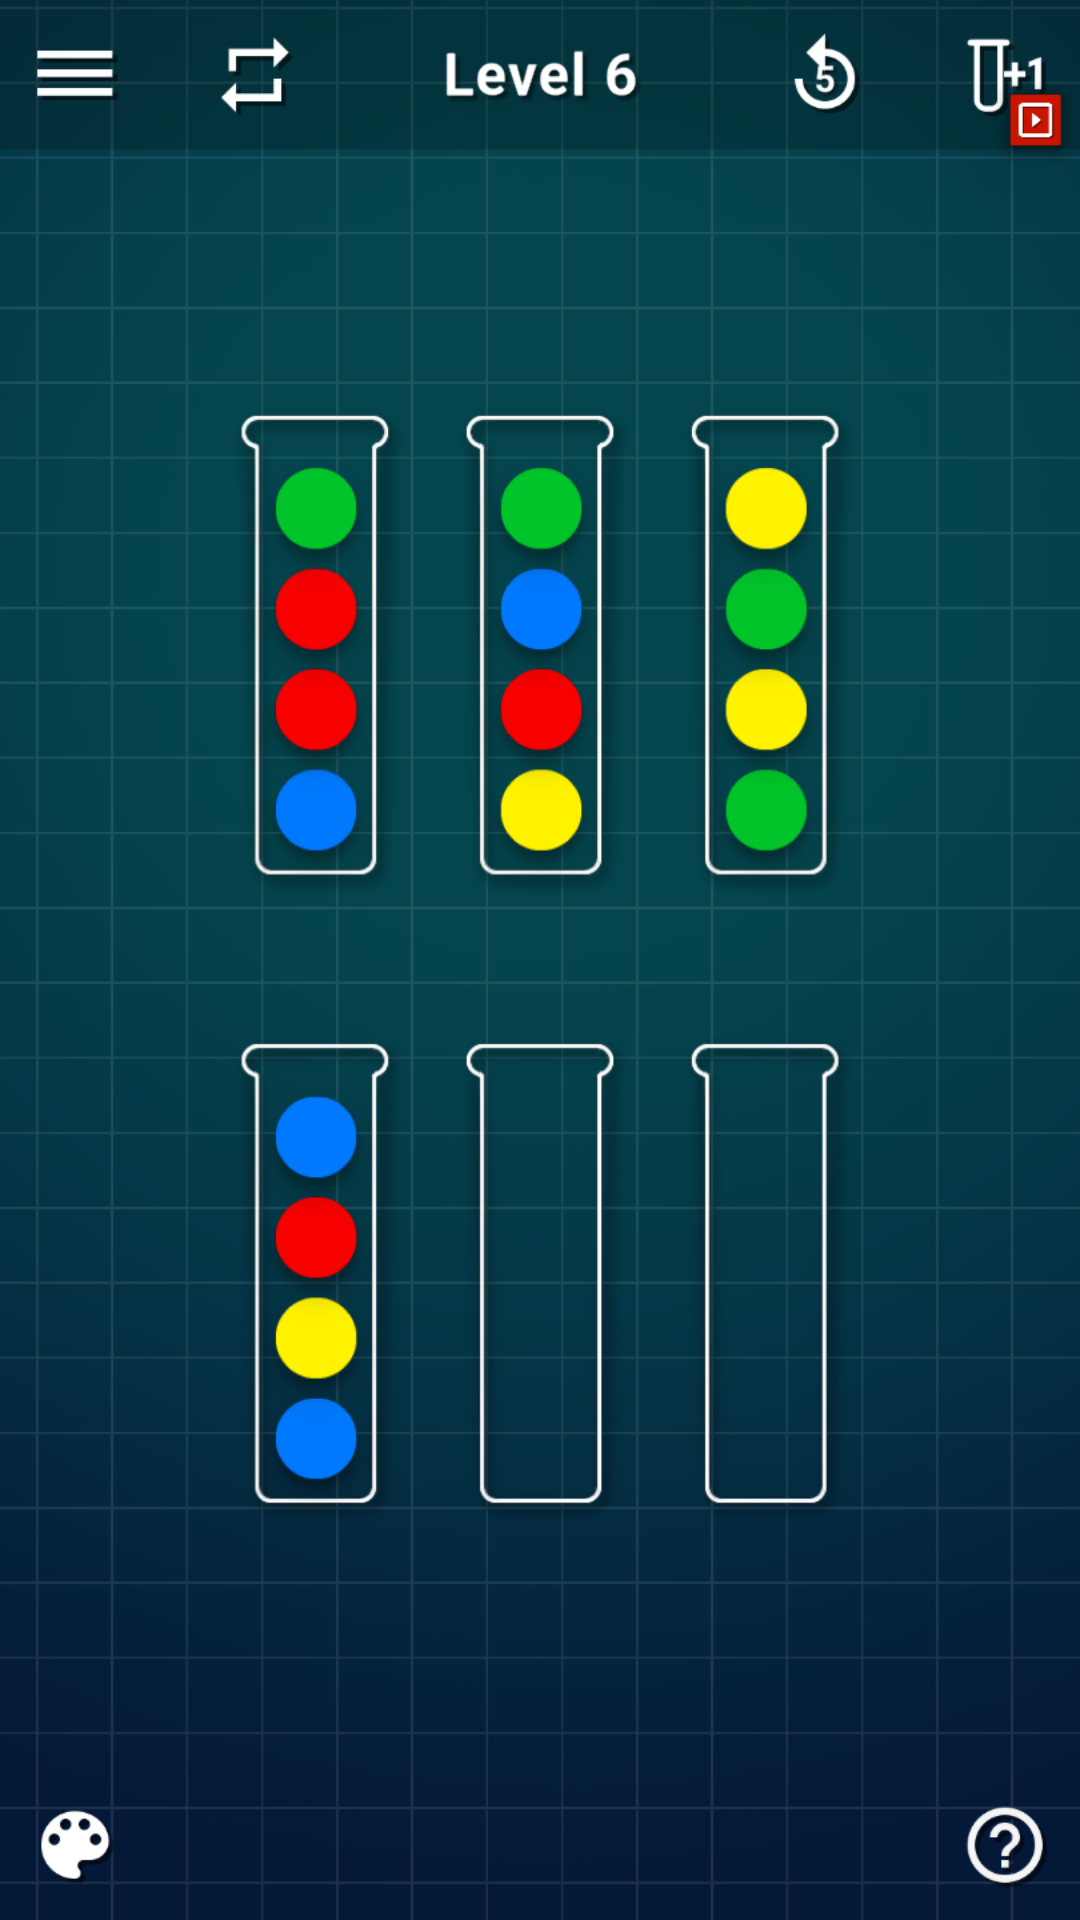
\includegraphics[width=29mm]{img/lvl6-begin.png}
  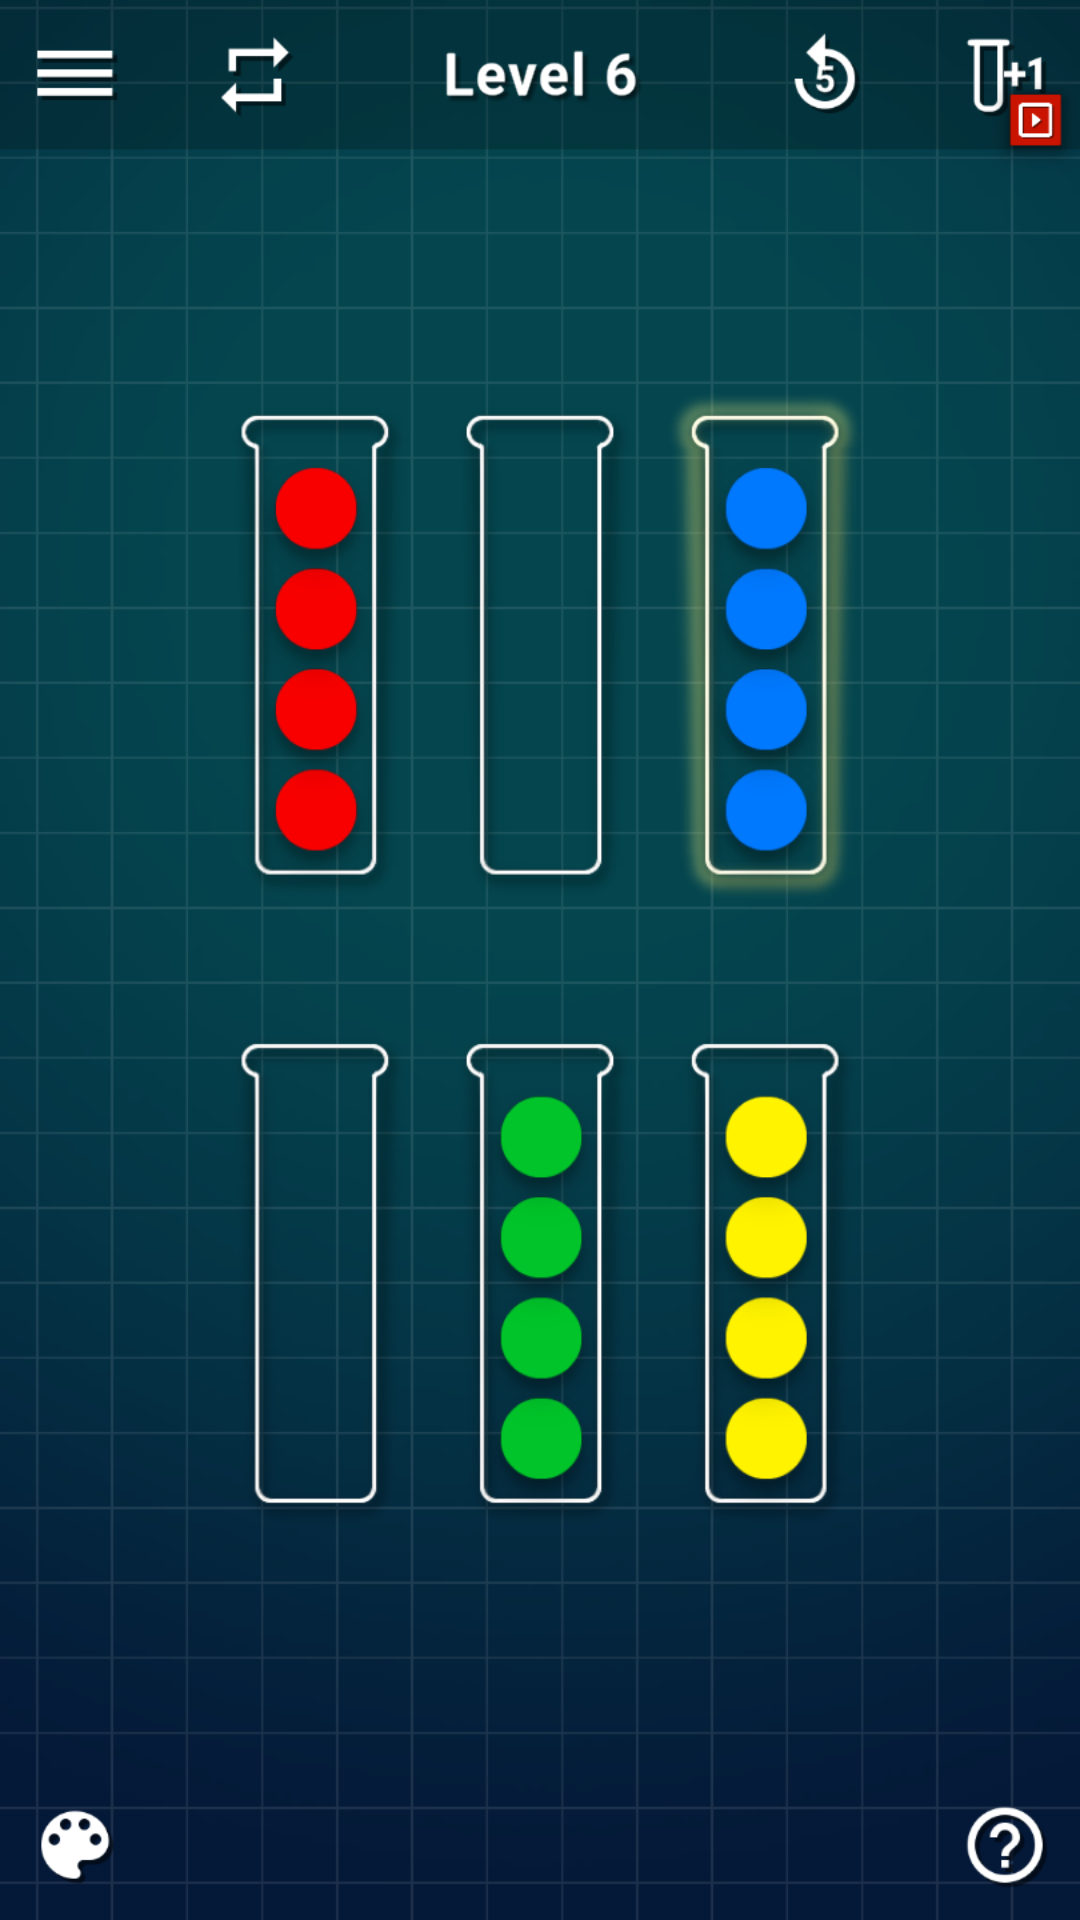
\includegraphics[width=29mm]{img/lvl6-end.png}
\end{minipage}

\end{frame}

\begin{frame}
\frametitle{Work specification}
\textbf{How we will solve it}

\begin{enumerate}
  \itemsep0em
  \item Implement the game
  \item Implement a human-friendly interface (if we have spare time).
  \item Use machine learning algorithms to solve the game, and compare performances. These algorithms are used to search for a path to a solution in a tree of game states.
\end{enumerate}

\end{frame}

\begin{frame}
\frametitle{Related works}

\end{frame}

\begin{frame}
  \frametitle{Tools and algorithms}
  \textbf{ML agents} | Reinforcement learning
  \begin{itemize}
    \item PPO (Proximal Policy Optimization)
    \item SAC (Soft-Actor Critic)
    \item POCA (Parallel Online Continuous Arcing), boosting (https://dl.acm.org/doi/10.5555/1597148.1597209)
  \end{itemize}
\end{frame}


\begin{frame}
\frametitle{Implementation (so far)}

\begin{itemize}
  \item \textbf{Language} | C\#
  \item \textbf{Environment} | Unity engine (v2020.2.2)
\end{itemize}

\textbf{Summary:} interface and puzzle generation implemented.

\begin{center}
  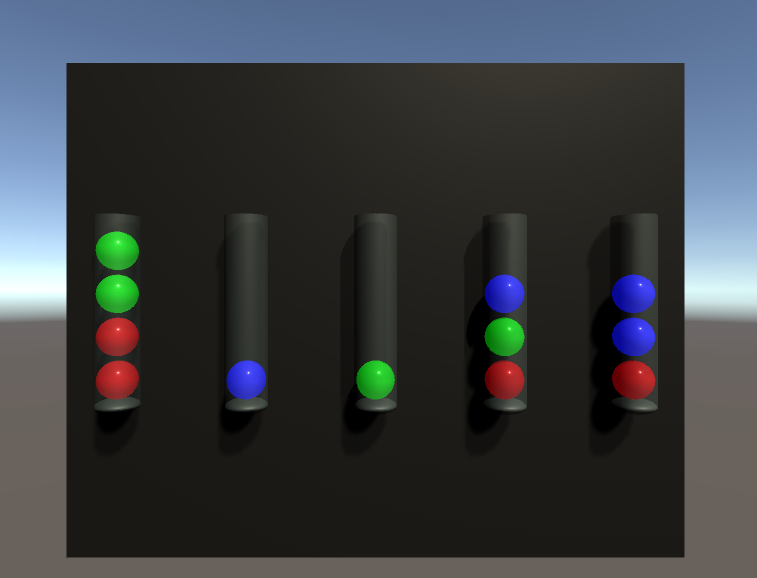
\includegraphics[width=75mm]{img/game-interface.png}
\end{center}

\end{frame}

\begin{frame}
  \frametitle{Bibliography}
  \setbeamertemplate{bibliography item}{\insertbiblabel}
  \bibliographystyle{acm}
  \bibliography{report}
  
\end{frame}

\end{document}
